% Recommender Systems Project Report: TopicLens
% Compile with pdfLaTeX, XeLaTeX or Tectonic (Overleaf: upload this folder, main file main.tex).

\documentclass[12pt,a4paper,oneside]{report}

\usepackage[T1]{fontenc}
\usepackage[utf8]{inputenc}
\usepackage{newtxtext,newtxmath}          % Times New Roman
\usepackage[a4paper,left=1.25in,right=1in,top=1in,bottom=1in]{geometry}
\usepackage{setspace}
\usepackage{graphicx}
\usepackage{booktabs}
\usepackage{array}
\usepackage{tabularx}
\usepackage{amsmath}
\usepackage{xcolor}
\usepackage{enumitem}
\usepackage{caption}
\usepackage{float}
\usepackage{titlesec}
\usepackage{tikz}
\usetikzlibrary{positioning,arrows.meta}
\usepackage[hidelinks]{hyperref}

% Details used on the title page
\newcommand{\reporttitle}{TopicLens}
\newcommand{\reportsubtitle}{An Explainable News Recommender}
\newcommand{\studentA}{Riddhima}
\newcommand{\regA}{2427010547}
\newcommand{\supervisor}{Pranshu Pranjal}
\newcommand{\acadyear}{2026--2027}

% Department guidelines: Times 12pt, justified, chapter and section headings bold 14pt,
% sub-headings italic 12pt, captions 10pt, page numbers bottom centre.
\onehalfspacing
\captionsetup{font=small,labelfont=bf}
\titleformat{\chapter}[block]{\normalfont\fontsize{14}{17}\bfseries\centering}{CHAPTER \thechapter:}{0.4em}{\MakeUppercase}
\titlespacing*{\chapter}{0pt}{0pt}{18pt}
\titleformat{\section}{\normalfont\fontsize{14}{17}\bfseries}{\thesection}{0.6em}{}
\titleformat{\subsection}{\normalfont\normalsize\itshape}{\thesubsection}{0.6em}{}
\setlist{itemsep=2pt,topsep=4pt}
\renewcommand{\contentsname}{Contents}
\renewcommand{\bibname}{References}
\newcolumntype{L}{>{\raggedright\arraybackslash}X}

\begin{document}

% ---------------------------------------------------------------- Title page
\pagenumbering{alph}
\begin{titlepage}
\begin{center}
\onehalfspacing
{\large Recommender Systems Project Report}\\[0.3cm]
{\large on}\\[0.6cm]
{\fontsize{24}{29}\selectfont\bfseries \reporttitle\par}
\vspace{0.2cm}
{\fontsize{14}{17}\selectfont \reportsubtitle\par}
\vspace{1cm}
{\large Submitted to Manipal University Jaipur}\\[0.2cm]
{\large Towards the partial fulfilment for the Award of the Degree of}\\[0.3cm]
{\fontsize{14}{17}\selectfont\bfseries B.\,Tech Computer Science and Engineering\\
(Artificial Intelligence and Machine Learning)\par}
\vspace{0.4cm}
{\large \acadyear}\\[1cm]
{\large By}\\[0.3cm]
{\fontsize{14}{17}\selectfont \studentA\\ \regA\par}
\vspace{1cm}

\includegraphics[height=0.9in,width=4.56in]{muj_logo.jpg}\\[1cm]
{\large Under the guidance of}\\[0.3cm]
{\fontsize{14}{17}\selectfont \supervisor\par}
\vspace{0.8cm}
{\large Department of Artificial Intelligence and Machine Learning}\\[0.2cm]
{\fontsize{16}{19}\selectfont\bfseries Manipal University Jaipur\\ Jaipur, Rajasthan\par}
\end{center}
\end{titlepage}

\pagenumbering{roman}

% ---------------------------------------------------------------- Abstract
\chapter*{ABSTRACT}
\addcontentsline{toc}{chapter}{ABSTRACT}

News apps decide what people read, but they rarely say why a story was chosen. When the feed gets it
wrong, the reader has no way to see the reason or correct it. The objective of this project is to build
TopicLens, a news recommender that ranks stories from a reader's click history, chosen topics, reactions
to earlier recommendations and direct feedback, and shows the exact reasons behind every pick.

TopicLens is trained on MIND-small, a public dataset of real, anonymised Microsoft News logs with 65,238
articles and 94,057 users. Topics are learned from the article text with non-negative matrix
factorisation, and ten features are built for every reader and article pair. Fourteen models were
trained and compared on the same time-based split, including KNN, linear and kernel SVMs, a random
forest, logistic regression, LightGBM and a neural model trained on a GPU.

On 73,152 test visits the models never saw, a hybrid of LightGBM and the neural model scored best with
an AUC of 66.60. Logistic regression reached 63.84, level with LightGBM and the linear SVM, while KNN
reached 55.66. The application uses the logistic regression, because its score splits exactly into
reasons that can be shown to the reader.

The result is a working web application built with React and TypeScript, with sign-in and storage on
Supabase. Every recommendation carries a one-line reason and an optional breakdown, and readers can
steer the feed with topic sliders, mutes and ``more or less like this''. The project shows that a simple,
fully explainable model gives up very little accuracy on this task.

\medskip
\noindent\textbf{Keywords:} news recommendation, explainable AI, MIND dataset, logistic regression,
topic modelling, Supabase

\clearpage
\tableofcontents
\clearpage

\pagenumbering{arabic}

% ================================================================ Chapter 1
\chapter{Introduction}

\section{Background and Motivation}
Most people now read news through a feed, and the order of that feed is set by a recommender system
trained on past clicks. These systems rank well, but they do not explain themselves. A reader cannot tell
whether a story is at the top because of their own reading, because it is popular or because it is new.
If the feed shows too much of one topic, there is usually no direct way to fix it.

Liu et al.\ \cite{liu2024} showed that topics learned from article text can be used to explain news
recommendations. TopicLens takes that idea and pairs it with a trained click model whose score can be
split exactly into its parts, so the explanation shown to the reader is the model's own reasoning and
not an approximation of it.

\section{Objectives of the Project}
\begin{itemize}
  \item Recommend news from four signals: reading and click history, preferred topics, interaction with
        earlier recommendations and explicit feedback.
  \item Train real machine learning models on a real dataset, including KNN and SVM, and compare them on
        one fixed train and test split.
  \item Pick a model that is accurate and whose score can be explained exactly.
  \item Show a short reason for every recommendation, with a detailed breakdown on request.
  \item Let readers sign in and keep their profile, preferences and history across devices.
\end{itemize}

\section{Scope of the Work}
In scope are: training and evaluating the models offline in Python; a web application with a ranked feed,
explanations, topic controls and feedback buttons; a topic explorer; a page that compares the trained
ranker with a simple baseline; and accounts with email, Google or guest sign-in.

Out of scope are: live news (the articles are from the MIND dataset, collected in November 2019), a
study with real users to measure trust, and running the neural model inside the browser.

\section{Product Scenarios}
\textbf{Scenario 1: A new reader.} Riya signs up with her email address and picks three sections she
likes: sports, health and movies. The feed opens with stories from those sections near the top, each
marked ``a section you chose''.

\textbf{Scenario 2: Asking why.} Riya sees a finance story ranked third and opens ``Why am I seeing
this?''. The panel shows that most of the score came from the story's popularity and its similarity to two
articles she read earlier, which are listed by name.

\textbf{Scenario 3: Pushing back.} She does not want finance news, so she drags the finance topic slider
to zero. The feed reorders at once, and a log shows which stories left her top ten.

\section{Organisation of the Report}
Chapter~2 covers the requirements and the method used to build and evaluate the models. Chapter~3
presents the system design: architecture, ranking model and database. Chapter~4 concludes the report and
lists the limitations and future work.

% ================================================================ Chapter 2
\chapter{Requirement Analysis}

\section{Functional Requirements}
\begin{table}[H]
\centering
\caption{Functional requirements}
\begin{tabularx}{\textwidth}{lL}
\toprule
ID & Requirement \\
\midrule
FR1 & A user can sign in with email and password, Google, or as a guest. \\
FR2 & A new user picks the news sections they like. \\
FR3 & The system shows a ranked feed of news stories for the user. \\
FR4 & Every story in the feed shows a one-line reason and an optional detailed breakdown. \\
FR5 & Opening a story counts as a click and updates the feed. \\
FR6 & The user can mark a story ``more like this'', ``less like this'' or ``not interested''. \\
FR7 & The user can raise, lower or mute any topic. \\
FR8 & The user's profile, preferences and interactions are saved and restored at next sign-in. \\
\bottomrule
\end{tabularx}
\end{table}

\section{Non-functional Requirements}
\begin{table}[H]
\centering
\caption{Non-functional requirements}
\begin{tabularx}{\textwidth}{lL}
\toprule
Type & Requirement \\
\midrule
Accuracy & The ranking model must clearly beat simple baselines on held-out data. \\
Explainability & The reasons shown must add up exactly to the model's score. \\
Speed & The feed must re-rank in under a second after any feedback. \\
Privacy & A user can only read and change their own data. \\
Cost & The system must run on free tiers and a single laptop GPU. \\
\bottomrule
\end{tabularx}
\end{table}

\section{Use Case Scenarios}
The two main use cases are getting a recommendation with its reasons, and giving feedback.
\begin{table}[H]
\centering
\caption{Use case: get and understand a recommendation}
\begin{tabularx}{\textwidth}{lL}
\toprule
Actor & Reader \\
Precondition & The reader is signed in and has picked sections. \\
Main flow & 1. The system ranks all candidate stories for the reader. 2. The reader opens ``Why am I seeing
this?'' on a story. 3. The system shows each signal's share of the score and the past reads behind it. \\
Result & The reader knows why the story was picked. \\
\bottomrule
\end{tabularx}
\end{table}

\begin{table}[H]
\centering
\caption{Use case: give feedback}
\begin{tabularx}{\textwidth}{lL}
\toprule
Actor & Reader \\
Precondition & The feed is shown. \\
Main flow & 1. The reader clicks ``less like this'' or lowers a topic slider. 2. The system updates the
scores and re-ranks the feed. 3. The change is saved to the database. \\
Result & The feed reflects the feedback, now and at the next sign-in. \\
\bottomrule
\end{tabularx}
\end{table}

\section{Methodology}

\subsection{Dataset}
The project uses MIND-small \cite{wu2020}, released by Microsoft Research for non-commercial research. It
has 65,238 news articles (title, abstract, category and subcategory), 94,057 anonymised users, 156,965
training visits from 9 to 14 November 2019 and 73,152 test visits from 15 November 2019. Each visit lists
the stories shown to a user and which ones they clicked. Only 4.05\% of shown stories were clicked, so the
models are judged on ranking metrics rather than plain accuracy.

\subsection{Train, validation and test split}
The split follows time so that no model sees the future. Models were fitted on visits from 9 to 13
November (126,695 visits), tuned on 14 November (30,270 visits) and tested once on the official test set
from 15 November (73,152 visits).

\subsection{Models compared}
Each model scores every shown story, and stories are sorted by score. The models were simple rules
(random, popularity, topic match, text match, category match), a KNN classifier ($k=50$), a linear SVM, a
kernel SVM, a random forest, logistic regression, LightGBM LambdaRank \cite{ke2017}, an NRMS-style neural
model \cite{wu2019} trained on an RTX 3050 GPU for 4 epochs, and a hybrid of LightGBM with the neural score
as an extra feature.

\subsection{Evaluation}
Four standard metrics were used \cite{wu2020}: AUC (how often a clicked story ranks above an unclicked
one; 50 is a coin flip), MRR (how high the first click sits) and nDCG@5 and nDCG@10 (how good the top 5
and top 10 are). Table~\ref{tab:results} shows the main results.

\begin{table}[H]
\centering
\caption{Results on the 73,152 test visits (higher is better)}
\label{tab:results}
\begin{tabular}{lcccc}
\toprule
Model & AUC & MRR & nDCG@5 & nDCG@10 \\
\midrule
Random & 50.07 & 21.91 & 22.38 & 28.66 \\
KNN classifier ($k=50$) & 55.66 & 25.97 & 27.85 & 34.00 \\
Popularity & 58.61 & 27.24 & 28.66 & 34.73 \\
Kernel SVM (RBF) & 60.40 & 27.86 & 30.27 & 36.82 \\
Random forest & 61.79 & 29.26 & 31.95 & 38.15 \\
Neural NRMS (GPU) & 63.14 & 29.75 & 32.20 & 38.64 \\
Linear SVM & 63.74 & 30.56 & 33.52 & 39.59 \\
LightGBM LambdaRank & 63.83 & 30.58 & 33.26 & 39.46 \\
Logistic regression (used in app) & 63.84 & 30.56 & 33.54 & 39.61 \\
\textbf{Hybrid: LightGBM + neural} & \textbf{66.60} & \textbf{32.05} & \textbf{35.47} & \textbf{41.64} \\
\midrule
BATM-NR, from \cite{liu2024} & 68.13 & 32.62 & 36.36 & 42.46 \\
\bottomrule
\end{tabular}
\end{table}

Logistic regression, the linear SVM and LightGBM finish within 0.1 AUC of each other, so the extra
complexity of trees buys almost nothing here. KNN does poorly because only 4\% of rows are clicks, so most
neighbours of any row are non-clicks. The hybrid is the most accurate, but it needs the neural encoder at
run time and cannot be explained exactly, so the application uses logistic regression.

% ================================================================ Chapter 3
\chapter{System Design}

\section{Design Goals}
\begin{itemize}
  \item \textbf{Recommendation first.} The feed is the main screen; explanations sit behind a single click.
  \item \textbf{Honest explanations.} Every reason shown is a real part of the model's score.
  \item \textbf{Instant feedback.} The model runs in the browser, so the feed re-ranks without a server
        round trip.
  \item \textbf{Simple to run.} One training script, static files and a managed database.
\end{itemize}

\section{System Architecture}
Training happens offline in Python. The script exports the articles, the topic model and the model
weights as JSON files, which the React application loads. Sign-in and storage go through Supabase
(Figure~\ref{fig:arch}).

\begin{figure}[H]
\centering
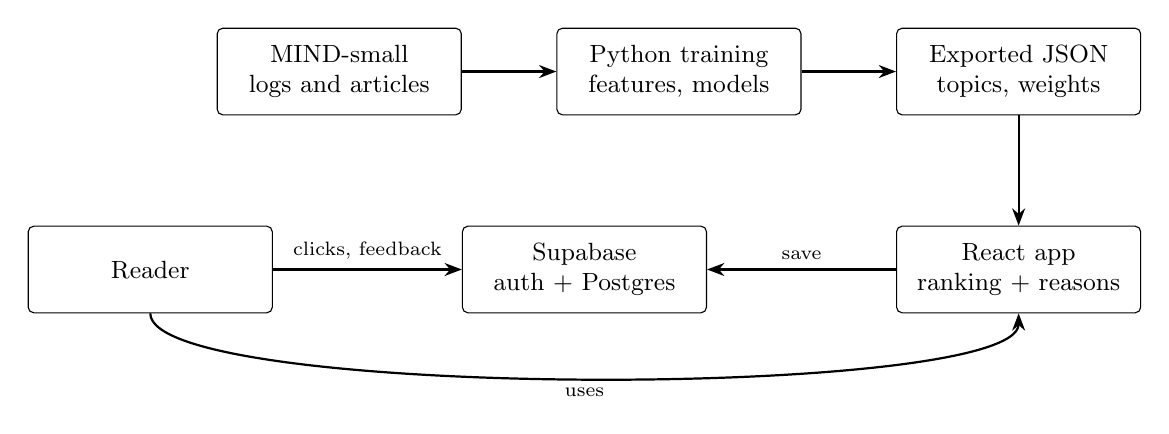
\begin{tikzpicture}[
  box/.style={draw, rounded corners=2pt, align=center, minimum width=3.1cm, minimum height=1.1cm, font=\small},
  arr/.style={-{Stealth[length=2.2mm]}, thick}]
  \node[box] (mind) {MIND-small\\logs and articles};
  \node[box, right=1.2cm of mind] (train) {Python training\\features, models};
  \node[box, right=1.2cm of train] (json) {Exported JSON\\topics, weights};
  \node[box, below=1.4cm of json] (app) {React app\\ranking + reasons};
  \node[box, left=2.4cm of app] (db) {Supabase\\auth + Postgres};
  \node[box, left=2.4cm of db] (user) {Reader};
  \draw[arr] (mind) -- (train);
  \draw[arr] (train) -- (json);
  \draw[arr] (json) -- (app);
  \draw[arr] (app) -- node[above, font=\scriptsize]{save} (db);
  \draw[arr] (user) -- node[above, font=\scriptsize]{clicks, feedback} (db);
  \draw[arr] (user.south) .. controls +(0,-1.1) and +(0,-1.1) .. node[below, font=\scriptsize]{uses} (app.south);
\end{tikzpicture}
\caption{System architecture of TopicLens}
\label{fig:arch}
\end{figure}

\begin{table}[H]
\centering
\caption{Technology stack}
\begin{tabularx}{\textwidth}{lL}
\toprule
Layer & Technology \\
\midrule
Machine learning & Python, pandas, scikit-learn \cite{pedregosa2011}, LightGBM, PyTorch with CUDA \\
Front end & React, TypeScript, Vite \\
Back end & Supabase: PostgreSQL, Auth, row-level security \\
Version control & Git and GitHub \\
\bottomrule
\end{tabularx}
\end{table}

\section{Detailed Design}

\subsection{Topics and features}
Each article's title and abstract are turned into TF-IDF vectors. Non-negative matrix factorisation
finds 30 topics, each described by its top words, and a 100-dimensional LSA space measures how close two
articles are in wording. For each reader and story, ten features are computed: topic match, text
similarity, category share, subcategory share, earlier-day clicks, earlier-day click rate, times shown
before, hours since publication, history length and number of stories shown together.

\subsection{Ranking and explanation}
The application scores each story with the trained logistic regression:
\begin{equation}
  s(u,a) = b + \sum_{j=1}^{10} w_j\, z_j(u,a)
\end{equation}
where $z_j$ is the $j$-th standardised feature for reader $u$ and story $a$. Each term $w_j z_j$ is shown as
that reason's share of the score, so the explanation adds up to the score by construction.

\subsection{How the four signals are used}
\begin{enumerate}
  \item \textbf{Click history:} opening a story adds it to the history, which updates the history-based
        features straight away.
  \item \textbf{Preferred sections:} chosen sections add $+2.0$ to the score of matching stories.
  \item \textbf{Earlier recommendations:} stories the reader skipped above a click lose $0.5$ per skip,
        up to three skips.
  \item \textbf{Explicit feedback:} more or less like this, not interested, topic sliders and mutes.
\end{enumerate}

\subsection{Database}
\begin{table}[H]
\centering
\caption{Main database tables}
\begin{tabularx}{\textwidth}{lL}
\toprule
Table & Contents \\
\midrule
profiles & Name, chosen sections and starting history for each user. \\
preferences & Topic sliders, mutes, liked, disliked and hidden stories, skip counts. \\
interactions & Append-only log of every click, read, like, dislike, dismiss and skip. \\
\bottomrule
\end{tabularx}
\end{table}

Row-level security lets each user see and change only their own rows, and the interaction log cannot be
edited or deleted by users.

% ================================================================ Chapter 4
\chapter{Conclusion}

\section{Conclusion}
TopicLens recommends news from a reader's history, chosen sections, skipped stories and direct feedback,
and explains every pick exactly. Of fourteen models tested on the same unseen data, the LightGBM and
neural hybrid was the most accurate at 66.60 AUC. Logistic regression scored 63.84, as good as LightGBM
and the linear SVM, and was chosen for the application because its reasons are exact.

\section{Limitations}
\begin{itemize}
  \item The news is from November 2019, so the app is a demonstration, not a live news service.
  \item The section boost and skip penalty were set by hand, not learned.
  \item No user study has been run yet, so the effect of explanations on trust is not measured.
\end{itemize}

\section{Future Work}
\begin{itemize}
  \item Run a small user study comparing the feed with and without explanations.
  \item Learn the feedback weights from the logged interactions.
  \item Bring part of the hybrid's accuracy into the app while keeping explanations exact.
\end{itemize}

% ================================================================ References
\begin{thebibliography}{9}
\addcontentsline{toc}{chapter}{REFERENCES}
\small\singlespacing

\bibitem{liu2024}
D. Liu, D. Greene, I. Li, X. Jiang and R. Dong, ``Topic-Centric Explanations for News Recommendation'',
\emph{ACM Transactions on Recommender Systems}, vol.~3, no.~2, 2024, doi:10.1145/3680295.

\bibitem{wu2020}
F. Wu, Y. Qiao, J.-H. Chen, C. Wu, T. Qi, J. Lian, D. Liu, X. Xie, J. Gao, W. Wu and M. Zhou,
``MIND: A Large-scale Dataset for News Recommendation'', in \emph{Proceedings of the 58th Annual Meeting of
the ACL}, 2020, pp.~3597--3606.

\bibitem{ke2017}
G. Ke, Q. Meng, T. Finley, T. Wang, W. Chen, W. Ma, Q. Ye and T.-Y. Liu, ``LightGBM: A Highly Efficient
Gradient Boosting Decision Tree'', in \emph{Advances in Neural Information Processing Systems 30}, 2017.

\bibitem{wu2019}
C. Wu, F. Wu, S. Ge, T. Qi, Y. Huang and X. Xie, ``Neural News Recommendation with Multi-Head
Self-Attention'', in \emph{Proceedings of EMNLP-IJCNLP}, 2019, pp.~6389--6394.

\bibitem{pedregosa2011}
F. Pedregosa et al., ``Scikit-learn: Machine Learning in Python'', \emph{Journal of Machine Learning
Research}, vol.~12, 2011, pp.~2825--2830.

\end{thebibliography}

\end{document}
